%==============================================================
%  EE201 -- Circuit Theory I
%  Lecture 9 : Trees, Cutsets and Fundamental Loops
%  M. Mert Ankaralı, METU EEE
%
%  Compile:  ./build.sh      (or: pdflatex EE201_Lecture_9.tex, twice)
%==============================================================
\documentclass[11pt,a4paper]{article}

%-------------------- packages --------------------------------
\usepackage[T1]{fontenc}
\usepackage[utf8]{inputenc}
\usepackage[english]{babel}
\usepackage{lmodern}
\usepackage[margin=2.3cm,top=2.0cm,bottom=1.9cm,headheight=14pt,headsep=9pt]{geometry}
\usepackage{amsmath,amssymb}
\usepackage{array,booktabs,tabularx}
\usepackage{enumitem}
\usepackage[table]{xcolor}
\usepackage{fancyhdr}
\usepackage{titlesec}
\usepackage{graphicx}
\usepackage[most]{tcolorbox}
\usepackage{tikz}
\usepackage[american,siunitx]{circuitikz}
\usetikzlibrary{matrix,arrows.meta,positioning,calc,decorations.pathmorphing,decorations.pathreplacing,decorations.markings,patterns,shapes.geometric}
\usepackage[colorlinks=true,allcolors=metured,breaklinks=true]{hyperref}

%-------------------- colour system ---------------------------
% One colour per physical quantity, used identically in the slides.
\definecolor{metured}{RGB}{155,27,48}    % headings, structure
\definecolor{metugray}{RGB}{88,89,91}
\definecolor{ccur}{RGB}{0,102,170}       % CURRENT  -- blue
\definecolor{cvolt}{RGB}{214,120,0}      % VOLTAGE  -- orange
\definecolor{cpow}{RGB}{23,128,74}       % POWER / ENERGY -- green
\definecolor{ccharge}{RGB}{124,60,160}   % CHARGE   -- purple
\definecolor{cflux}{RGB}{0,138,138}      % FLUX -- teal
\definecolor{boxgray}{RGB}{245,245,245}
\definecolor{copper}{RGB}{184,98,30}

\newcommand{\Icol}[1]{\textcolor{ccur}{#1}}
\newcommand{\Vcol}[1]{\textcolor{cvolt}{#1}}
\newcommand{\Pcol}[1]{\textcolor{cpow}{#1}}
\newcommand{\Qcol}[1]{\textcolor{ccharge}{#1}}
\newcommand{\Fcol}[1]{\textcolor{cflux}{#1}}

%-------------------- units (no siunitx dependency) -----------
\newcommand{\uni}[1]{\,\mathrm{#1}}
\newcommand{\A}{\uni{A}}   \newcommand{\V}{\uni{V}}
\newcommand{\W}{\uni{W}}   \newcommand{\J}{\uni{J}}
\newcommand{\Cb}{\uni{C}}  \newcommand{\s}{\uni{s}}
\newcommand{\Sie}{\uni{S}} \newcommand{\Wb}{\uni{Wb}}

%-------------------- layout ----------------------------------
\pagestyle{fancy}
\fancyhf{}
\lhead{\small\textcolor{metugray}{EE201 -- Circuit Theory I}}
\rhead{\small\textcolor{metugray}{Lecture 9: Trees, Cutsets and Fundamental Loops}}
\cfoot{\small\thepage}
\renewcommand{\headrulewidth}{0.4pt}

\titleformat{\section}{\large\bfseries\color{metured}}{\thesection.}{0.6em}{}
\titleformat{\subsection}{\normalsize\bfseries\color{metugray}}{\thesubsection.}{0.6em}{}
\titlespacing*{\section}{0pt}{1.4ex plus .3ex}{0.7ex}
\titlespacing*{\subsection}{0pt}{1.1ex plus .2ex}{0.5ex}

\setlist[itemize]{itemsep=2pt,topsep=3pt,parsep=0pt,leftmargin=1.5em}
\setlist[enumerate]{itemsep=2pt,topsep=3pt,parsep=0pt,leftmargin=1.7em}
\setlength{\parindent}{0pt}
\setlength{\parskip}{0.7ex plus .1ex}
\raggedbottom
\widowpenalty=10000
\clubpenalty=10000
\brokenpenalty=10000

%-------------------- boxes -----------------------------------
\newtcolorbox{definitionbox}[1]{enhanced,
  colback=metured!4, colframe=metured, boxrule=0.9pt,
  fonttitle=\bfseries, title={#1}, arc=2pt,
  left=7pt,right=7pt,top=5pt,bottom=5pt, before skip=7pt, after skip=7pt,
  before upper={\setlength{\parskip}{0.6ex plus .1ex}}}

\newtcolorbox{ideabox}[1][Key idea]{enhanced,
  colback=ccur!5, colframe=ccur, boxrule=0.9pt,
  fonttitle=\bfseries, title={#1}, arc=2pt,
  left=7pt,right=7pt,top=5pt,bottom=5pt, before skip=7pt, after skip=7pt,
  before upper={\setlength{\parskip}{0.6ex plus .1ex}}}

\newtcolorbox{examplebox}[1][Example]{enhanced,
  colback=cpow!4, colframe=cpow, boxrule=0.9pt,
  fonttitle=\bfseries, title={#1}, arc=2pt,
  left=7pt,right=7pt,top=5pt,bottom=5pt, before skip=7pt, after skip=7pt,
  before upper={\setlength{\parskip}{0.6ex plus .1ex}}}

\newtcolorbox{cautionbox}[1][Careful]{enhanced,
  colback=cvolt!6, colframe=cvolt, boxrule=0.9pt,
  fonttitle=\bfseries, title={#1}, arc=2pt,
  left=7pt,right=7pt,top=5pt,bottom=5pt, before skip=7pt, after skip=7pt,
  before upper={\setlength{\parskip}{0.6ex plus .1ex}}}

%-------------------- circuitikz defaults ---------------------
\ctikzset{bipoles/length=0.9cm, color=black,
          label/align=straight,
          bipoles/generic/height=0.28, bipoles/generic/width=0.62}
\tikzset{
  iar/.style={-{Stealth[length=2.2mm]}, ccur, thick},
  pol/.style={font=\small, text=cvolt},
  glab/.style={font=\footnotesize, text=metured},
  ttl/.style={font=\scriptsize\bfseries, text=metugray},
  capn/.style={font=\scriptsize, text=metugray, align=center},
  bigarr/.style={-{Stealth[length=3mm]}, very thick, metugray},
  gnode/.style={circle, fill=metured, inner sep=0pt, minimum size=4.4pt},
  nlab/.style={circle, draw=metured, text=metured, font=\scriptsize, inner sep=0.7pt},
  blab/.style={font=\footnotesize, text=black!80},
  gbr/.style={black!75, thick, postaction={decorate, decoration={markings,
      mark=at position 0.56 with {\arrow{Stealth[length=2.5mm]}}}}},
  hal/.style={draw=cpow!60, line width=6pt, opacity=0.35, line cap=round, line join=round},
  elem/.style={draw=metugray, thick, fill=metulight},
}
\definecolor{metulight}{RGB}{243,240,241}
\newcommand{\ohm}{\,\Omega}

%  A circled node number, for the text and the matrices
\newcommand{\nd}[1]{\tikz[baseline=(c.base)]\node[nlab](c){#1};}
%  Branch current arrow beside the element from #1 to #2, on side #3 (90 = left, -90 = right),
%  with branch number #4
\newcommand{\brarr}[4]{%
  \draw[iar] ($(#1)!0.34!(#2)!0.34cm!#3:(#2)$) -- ($(#1)!0.66!(#2)!0.34cm!#3:(#2)$);
  \node[blab] at ($(#1)!0.5!(#2)!0.66cm!#3:(#2)$) {#4};}
%  A straight graph branch from #1 to #2, number #4 on side #3
\newcommand{\gbranch}[4]{%
  \draw[gbr] (#1) -- (#2);
  \node[blab] at ($(#1)!0.5!(#2)!0.28cm!#3:(#2)$) {#4};}
%  An incidence matrix with node labels on the left and branch numbers on top.
%  #1 name, #2 number of columns, #3 node labels, #4 rows (entries separated by \&)
\newcommand{\incmat}[4]{%
  \begin{tikzpicture}[baseline={([yshift=-0.6ex]#1.center)}]
    \matrix (#1) [matrix of math nodes, ampersand replacement=\&,
                  left delimiter={[}, right delimiter={]}, inner sep=1pt,
                  column sep=0.45em,
                  nodes={text width=1.35em, align=right, minimum height=1.25em,
                         inner sep=1pt}] {#4};
    \foreach \j in {1,...,#2}
      \node[font=\scriptsize, text=metugray, anchor=south east, inner sep=1pt]
        at ([yshift=2pt]#1-1-\j.north east) {\j};
    \foreach \lab [count=\i] in {#3}
      \node[nlab, left=11pt] at (#1.west |- #1-\i-1) {\lab};
  \end{tikzpicture}}
%  Same, with explicit column labels: #1 name, #2 column labels, #3 row labels,
%  #4 rows, #5 extra TikZ code
\newcommand{\incmatc}[5]{%
  \begin{tikzpicture}[baseline={([yshift=-0.6ex]#1.center)}]
    \matrix (#1) [matrix of math nodes, ampersand replacement=\&,
                  left delimiter={[}, right delimiter={]}, inner sep=1pt,
                  column sep=0.45em,
                  nodes={text width=1.35em, align=right, minimum height=1.25em,
                         inner sep=1pt}] {#4};
    \foreach \lab [count=\j] in {#2}
      \node[font=\scriptsize, text=metugray, anchor=south east, inner sep=1pt]
        at ([yshift=2pt]#1-1-\j.north east) {\lab};
    \foreach \lab [count=\i] in {#3}
      \node[nlab, left=11pt] at (#1.west |- #1-\i-1) {\lab};
    #5
  \end{tikzpicture}}
%  A two-winding ideal-transformer symbol between (#1,0)--(#1,#2) on the left and
%  (#1+1.6,0)--(#1+1.6,#2) on the right; dots at the top of both windings.
\newcommand{\xfmr}[2]{%
  \begin{scope}[xshift=#1 cm]
    \ctikzset{bipoles/length=1.35cm}
    \draw (0,0) to[L] (0,#2);
    \draw (1.6,#2) to[L] (1.6,0);
    \draw[line width=1.1pt, metugray] (0.72,-0.05) -- (0.72,#2+0.05);
    \draw[line width=1.1pt, metugray] (0.88,-0.05) -- (0.88,#2+0.05);
    \fill (0.36,#2-0.2) circle (2.1pt);
    \fill (1.24,#2-0.2) circle (2.1pt);
  \end{scope}}
%  The four node positions of the bridge circuit N
\newcommand{\bridgecoords}{%
  \coordinate (n1) at (0,1.7);  \coordinate (n2) at (-1.5,0);
  \coordinate (n3) at (1.5,0);  \coordinate (n4) at (0,-1.7);}
\newcommand{\bridgenodes}{%
  \foreach \k/\pos in {1/above, 2/left, 3/right, 4/below}
    {\fill[metured] (n\k) circle (2.2pt); \node[nlab, \pos=3pt] at (n\k) {\k};}}

\newcommand{\bridgegraph}{%
  \gbranch{n1}{n2}{-90}{1}  \gbranch{n1}{n3}{90}{2}  \gbranch{n3}{n2}{-90}{3}
  \gbranch{n2}{n4}{-90}{4}  \gbranch{n3}{n4}{90}{5}
  \draw[gbr] (n4) to[out=180, in=180, looseness=2.3] (n1);
  \node[blab] at (-2.55,0) {6};
  \bridgenodes}

%  A graph branch from #1 to #2 with its branch voltage: + near the tail, - near the head,
%  v_#4 in the middle; #3 = auto=left or auto=right picks the side
\newcommand{\gvbranch}[4]{%
  \draw[gbr] (#1) --
    node[pos=0.27, #3, pol, inner sep=1pt] {$+$}
    node[pos=0.5, #3, font=\small, text=cvolt, inner sep=2.5pt] {$v_{#4}$}
    node[pos=0.73, #3, pol, inner sep=1pt] {$-$} (#2);}
\newcommand{\bridgevgraph}{%
  \gvbranch{n1}{n2}{auto=right}{1}  \gvbranch{n1}{n3}{auto=left}{2}
  \gvbranch{n3}{n2}{auto=right}{3}  \gvbranch{n2}{n4}{auto=right}{4}
  \gvbranch{n3}{n4}{auto=left}{5}
  \draw[gbr] (n4) to[out=180, in=180, looseness=2.3]
    node[pos=0.22, left, pol, inner sep=2pt] {$+$}
    node[pos=0.5, left, font=\small, text=cvolt] {$v_6$}
    node[pos=0.78, left, pol, inner sep=2pt] {$-$} (n1);
  \bridgenodes}
%  One branch, for the definition: + at the tail, - at the head, current along the arrow
\newcommand{\onebranch}{%
  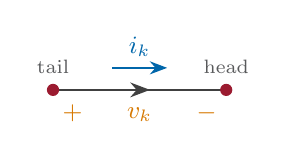
\begin{tikzpicture}[baseline=-0.6ex]
    \coordinate (p) at (0,0); \coordinate (q) at (2.2,0);
    \draw[gbr] (p) -- (q);
    \fill[metured] (p) circle (2.2pt); \fill[metured] (q) circle (2.2pt);
    \node[pol] at (0.25,-0.3) {$+$}; \node[pol] at (1.95,-0.3) {$-$};
    \node[font=\small, text=cvolt] at (1.1,-0.32) {$v_k$};
    \draw[iar] (0.75,0.28) -- (1.45,0.28); \node[font=\small, text=ccur] at (1.1,0.55) {$i_k$};
    \node[font=\scriptsize, text=metugray] at (0,0.3) {tail};
    \node[font=\scriptsize, text=metugray] at (2.2,0.3) {head};
  \end{tikzpicture}}

%==============================================================
%-------------------- Lecture 8 additions ---------------------
\tikzset{mlabst/.style={draw=ccur, text=ccur, fill=white, rounded corners=1.5pt,
                        inner sep=1.2pt, font=\scriptsize\bfseries}}
%  A boxed mesh number, for the text
\newcommand{\mlab}[1]{\tikz[baseline=(c.base)]\node[mlabst](c){#1};}
%  A clockwise mesh arrow at (#2,#3) with mesh number #4; optional radius #1
\newcommand{\meshcw}[4][0.32]{%
  \draw[ccur, thick, -{Stealth[length=2mm]}] ($(#2,#3)+(150:#1)$)
    arc[start angle=150, end angle=-150, radius=#1];
  \node[mlabst] at (#2,#3) {#4};}
%  The three inner meshes of the bridge graph (after \bridgecoords)
\newcommand{\bridgemeshes}{%
  \meshcw[0.3]{0}{0.82}{1} \meshcw[0.3]{0}{-0.78}{2} \meshcw[0.24]{-1.55}{0.66}{3}}
\newcommand{\fillmeshA}[1][]{\fill[ccur!14, #1] (n1) -- (n2) -- (n3) -- cycle;}
\newcommand{\fillmeshB}[1][]{\fill[ccur!14, #1] (n2) -- (n3) -- (n4) -- cycle;}
\newcommand{\fillmeshC}[1][]{\fill[ccur!14, #1] (n4) to[out=180, in=180, looseness=2.3] (n1) -- (n2) -- cycle;}
%  The bridge graph drawn as a square: both diagonals cross
%  Separable / nonseparable pictures: before and after removing one node.
%  Removed node: open grey circle; removed branches: dashed grey.
\tikzset{gone/.style={gray!55, thick, dash pattern=on 2.5pt off 2pt},
  gonenode/.style={gray!70, thick, fill=white},
  gonelab/.style={nlab, draw=gray!70, text=gray!70}}
\newcommand{\twotricoords}{%
  \coordinate (c) at (1.6,0.8);
  \coordinate (a1) at (0,1.6); \coordinate (a2) at (0,0);
  \coordinate (b1) at (3.2,1.6); \coordinate (b2) at (3.2,0);}
\newcommand{\twotri}{%
  \twotricoords
  \draw[black!75, thick] (c) -- (a1) -- (a2) -- cycle;
  \draw[black!75, thick] (c) -- (b1) -- (b2) -- cycle;
  \foreach \p in {a1,a2,b1,b2,c} \fill[metured] (\p) circle (2.2pt);}
\newcommand{\twotricut}{%
  \twotricoords
  \draw[gone] (a1) -- (c) -- (a2);  \draw[gone] (b1) -- (c) -- (b2);
  \draw[cvolt, very thick] (a1) -- (a2);  \draw[ccur, very thick] (b1) -- (b2);
  \foreach \p in {a1,a2,b1,b2} \fill[metured] (\p) circle (2.2pt);
  \draw[gonenode] (c) circle (2.6pt);}
%  N with node 2 removed: branches 1, 3, 4 go; 2, 5, 6 stay (one piece)
\newcommand{\bridgecut}{%
  \bridgecoords
  \draw[gone] (n1) -- (n2);  \draw[gone] (n3) -- (n2);  \draw[gone] (n2) -- (n4);
  \begin{scope}[gbr/.append style={ccur, very thick}]
    \gbranch{n1}{n3}{90}{2}  \gbranch{n3}{n4}{90}{5}
    \draw[gbr] (n4) to[out=180, in=180, looseness=2.3] (n1);
  \end{scope}
  \node[blab] at (-2.55,0) {6};
  \foreach \k/\pos in {1/above, 3/right, 4/below}
    {\fill[metured] (n\k) circle (2.2pt); \node[nlab, \pos=3pt] at (n\k) {\k};}
  \draw[gonenode] (n2) circle (2.6pt);
  \node[gonelab, left=3pt] at (n2) {2};}
%  Separable vs nonseparable, before and after removing a node. #1, #3: extra options
%  for the two "after" pictures; #2, #4: for the removed parts drawn in them
%  (overlay styles on slides, empty in the notes)
\newcommand{\nsepfigure}[4]{%
  \begin{tikzpicture}[scale=0.8]
    \begin{scope}
      \twotri
      \node[ttl] at (1.6,-1.2) {separable};
    \end{scope}
    \begin{scope}[#1]
      \draw[bigarr] (3.6,0.8) -- (4.4,0.8);
      \node[capn] at (4.0,1.35) {remove\\ centre};
      \begin{scope}[xshift=4.8cm, gone/.append style={#2}, gonenode/.append style={#2}]
        \twotricut
      \end{scope}
      \node[ttl] at (6.4,-1.2) {\textcolor{cvolt}{two} \textcolor{ccur}{pieces}};
    \end{scope}
    \draw[metugray!50] (8.7,-1.4) -- (8.7,2.3);
    \begin{scope}[xshift=11.0cm, yshift=0.8cm, scale=0.75, transform shape]
      \bridgecoords \bridgegraph
    \end{scope}
    \node[ttl] at (10.6,-1.2) {nonseparable (bridge)};
    \begin{scope}[#3]
      \draw[bigarr] (12.55,0.8) -- (13.45,0.8);
      \node[capn] at (13.0,1.35) {remove\\ node 2};
      \begin{scope}[xshift=15.9cm, yshift=0.8cm, scale=0.75, transform shape,
                    gone/.append style={#4}, gonenode/.append style={#4},
                    gonelab/.append style={#4}]
        \bridgecut
      \end{scope}
      \node[ttl] at (15.5,-1.2) {\textcolor{ccur}{still one piece}};
    \end{scope}
  \end{tikzpicture}}
\newcommand{\squarekfour}{%
  \coordinate (s1) at (0,2); \coordinate (s3) at (2,2);
  \coordinate (s4) at (2,0); \coordinate (s2) at (0,0);
  \foreach \u/\v/\k/\lp in {s1/s2/1/left, s1/s3/2/above, s2/s4/4/below, s3/s4/5/right}
    \draw[black!75, thick] (\u) -- (\v) node[midway, \lp, blab] {\k};
  \draw[black!75, thick] (s3) -- (s2) node[pos=0.25, above left, blab, inner sep=1pt] {3};
  \draw[black!75, thick] (s4) -- (s1) node[pos=0.25, above right, blab, inner sep=1pt] {6};
  \foreach \k/\pos in {1/above left, 2/below left, 3/above right, 4/below right}
    {\fill[metured] (s\k) circle (2.2pt); \node[nlab, \pos=1pt] at (s\k) {\k};}}
%  The circuit of the Tellegen example (10 V, 2, 4, 12 ohm), with current references
%  A hop (bump): the wire passes over another one without touching it.
%  \hopseg{P}{X}{Q}: from P to Q, jumping at the crossing point X
\newcommand{\hopr}{0.22cm}
\newcommand{\hopseg}[3]{%
  ($(#2)!\hopr!(#1)$) to[bend left=90, looseness=1.55] ($(#2)!\hopr!(#3)$)}
%  The square drawing of the bridge graph, branch 6 hopping over branch 3
\newcommand{\squarehop}{%
  \coordinate (s1) at (0,2); \coordinate (s3) at (2,2);
  \coordinate (s4) at (2,0); \coordinate (s2) at (0,0);
  \coordinate (sx) at (1,1);
  \foreach \u/\v/\k/\lp in {s1/s2/1/left, s1/s3/2/above, s2/s4/4/below, s3/s4/5/right}
    \draw[black!75, thick] (\u) -- (\v) node[midway, \lp, blab] {\k};
  \draw[black!75, thick] (s3) -- (s2) node[pos=0.25, above left, blab, inner sep=1pt] {3};
  \draw[copper, very thick] (s4) -- \hopseg{s4}{sx}{s1} -- (s1);
  \node[blab, text=copper] at (1.62,0.62) {6};
  \foreach \k/\pos in {1/above left, 2/below left, 3/above right, 4/below right}
    {\fill[metured] (s\k) circle (2.2pt); \node[nlab, \pos=1pt] at (s\k) {\k};}}
%  The nonplanar hexagon graph with as few hops as possible: one diagonal goes around
%  the outside, and one hop is still left
\newcommand{\hexhop}{%
  \foreach \a/\n in {0/a,60/b,120/c,180/d,240/e,300/f} \coordinate (\n) at (\a:1.15);
  \draw[black!75, thick] (a) -- (b) -- (c) -- (d) -- (e) -- (f) -- cycle;
  \draw[black!75, thick] (a) -- (d);
  \draw[black!75, thick] (b) .. controls (3.1,2.2) and (0.6,-3.3) .. (e);
  \draw[copper, very thick] (c) -- \hopseg{c}{0,0}{f} -- (f);
  \foreach \n in {a,b,c,d,e,f} \fill[metured] (\n) circle (2.2pt);}
%  The same graph in 3D: hexagon on a board, diagonals lifted to different heights.
%  #1: the x, y, z unit vectors of the view
\newcommand{\hexthreeD}[1]{%
  \begin{scope}[#1]
    \fill[metulight] (-1.55,-1.55,0) -- (1.55,-1.55,0) -- (1.55,1.55,0) -- (-1.55,1.55,0) -- cycle;
    \draw[gray!45] (-1.55,-1.55,0) -- (1.55,-1.55,0) -- (1.55,1.55,0) -- (-1.55,1.55,0) -- cycle;
    \foreach \a in {0,60,...,300}
      \draw[black!75, thick] ({1.15*cos(\a)},{1.15*sin(\a)},0) -- ({1.15*cos(\a+60)},{1.15*sin(\a+60)},0);
    \draw[black!75, thick] ({1.15*cos(120)},{1.15*sin(120)},0) -- ({-1.15*cos(120)},{-1.15*sin(120)},0);
    \foreach \a/\h in {0/0.6, 60/1.15}
      \draw[copper, very thick] plot[domain=0:1, samples=31, variable=\t]
        ({1.15*cos(\a)*(1-2*\t)},{1.15*sin(\a)*(1-2*\t)},{\h*sin(180*\t)});
    \foreach \a in {0,60,...,300} \fill[metured] ({1.15*cos(\a)},{1.15*sin(\a)},0) circle (2.2pt);
  \end{scope}}
\tikzset{
  view top/.style={x={(1cm,0cm)}, y={(0cm,1cm)}, z={(0cm,0cm)}},
  view oblique/.style={x={(0.9cm,-0.32cm)}, y={(0.9cm,0.32cm)}, z={(0cm,0.95cm)}},
  view side/.style={x={(1cm,0cm)}, y={(0.22cm,0.1cm)}, z={(0cm,0.95cm)}},
}
\newcommand{\tcircuit}[1]{%
\begin{tikzpicture}[scale=#1]
  \draw (0,0) to[american voltage source, invert] (0,2.2);
  \node[font=\small, left] at (-0.45,1.1) {$10\V$};
  \draw (0,2.2) to[R] (2.6,2.2);
  \node[font=\small] at (1.3,2.62) {$2\ohm$};
  \draw (2.6,2.2) -- (4.4,2.2);
  \draw (2.6,2.2) to[R] (2.6,0);
  \node[font=\small, right] at (2.85,1.75) {$4\ohm$};
  \draw (4.4,2.2) to[R] (4.4,0);
  \node[font=\small, right] at (4.65,1.1) {$12\ohm$};
  \draw (4.4,0) -- (0,0);
  \draw[iar] (0.55,0.7) -- (0.55,1.5);  \node[font=\small, text=ccur] at (0.85,1.1) {$i_1$};
  \draw[iar] (0.85,1.8) -- (1.75,1.8);  \node[font=\small, text=ccur] at (1.3,1.5) {$i_2$};
  \draw[iar] (2.25,1.45) -- (2.25,0.75); \node[font=\small, text=ccur] at (1.95,1.1) {$i_3$};
  \draw[iar] (4.05,1.45) -- (4.05,0.75); \node[font=\small, text=ccur] at (3.75,1.1) {$i_4$};
  \foreach \x/\y/\k/\pos in {0/2.2/1/above left, 2.6/2.2/2/above, 1.3/0/3/below}
    {\fill[metured] (\x,\y) circle (2.2pt); \node[nlab, \pos=2pt] at (\x,\y) {\k};}
  \meshcw[0.28]{1.3}{0.65}{1}
  \meshcw[0.28]{3.3}{0.6}{2}
\end{tikzpicture}}
%  A mesh matrix: like \incmat, with mesh numbers as row labels
\newcommand{\incmatm}[4]{%
  \begin{tikzpicture}[baseline={([yshift=-0.6ex]#1.center)}]
    \matrix (#1) [matrix of math nodes, ampersand replacement=\&,
                  left delimiter={[}, right delimiter={]}, inner sep=1pt,
                  column sep=0.45em,
                  nodes={text width=1.35em, align=right, minimum height=1.25em,
                         inner sep=1pt}] {#4};
    \foreach \j in {1,...,#2}
      \node[font=\scriptsize, text=metugray, anchor=south east, inner sep=1pt]
        at ([yshift=2pt]#1-1-\j.north east) {\j};
    \foreach \lab [count=\i] in {#3}
      \node[mlabst, left=11pt] at (#1.west |- #1-\i-1) {\lab};
  \end{tikzpicture}}
%  Slides only: the mesh matrix of N, row k shown from overlay k+1 on
\newcommand{\incmatmv}[4]{%
  \begin{tikzpicture}[baseline={([yshift=-0.6ex]#1.center)}]
    \matrix (#1) [matrix of math nodes, ampersand replacement=\&,
                  left delimiter={[}, right delimiter={]}, inner sep=1pt,
                  column sep=0.45em,
                  nodes={text width=1.35em, align=right, minimum height=1.25em,
                         inner sep=1pt},
                  row 1/.style={nodes={visible on=<2->}},
                  row 2/.style={nodes={visible on=<3->}},
                  row 3/.style={nodes={visible on=<4->}}] {#4};
    \foreach \j in {1,...,#2}
      \node[font=\scriptsize, text=metugray, anchor=south east, inner sep=1pt]
        at ([yshift=2pt]#1-1-\j.north east) {\j};
    \foreach \lab [count=\i] in {#3}
      \node[mlabst, left=11pt] at (#1.west |- #1-\i-1) {\lab};
  \end{tikzpicture}}

%==============================================================
%-------------------- Lecture 9 additions ---------------------
\definecolor{ctree}{RGB}{23,128,74}      % tree branches -- green
\tikzset{
  treebr/.style={gbr, ctree, line width=2.1pt},
  cotreebr/.style={gbr},
  hlbr/.style={gbr, cvolt, line width=2.1pt},
  faintbr/.style={black!22, thick},
  plainbr/.style={black!75, thick},
  surf/.style={cvolt, thick, dash pattern=on 3pt off 2pt},
}
%  A straight branch from #1 to #2, number #4 on side #3, drawn with style #5
\newcommand{\sbranch}[5]{%
  \draw[#5] (#1) -- (#2);
  \node[blab] at ($(#1)!0.5!(#2)!0.28cm!#3:(#2)$) {#4};}
%  The bridge graph with a style for each of its six branches
\newcommand{\bridgesub}[6]{%
  \sbranch{n1}{n2}{-90}{1}{#1}  \sbranch{n1}{n3}{90}{2}{#2}  \sbranch{n3}{n2}{-90}{3}{#3}
  \sbranch{n2}{n4}{-90}{4}{#4}  \sbranch{n3}{n4}{90}{5}{#5}
  \draw[#6] (n4) to[out=180, in=180, looseness=2.3] (n1);
  \node[blab] at (-2.55,0) {6};
  \bridgenodes}
%  The graph G of this lecture: 4 nodes, 6 branches (branch 5 curved, parallel to 4)
\newcommand{\tgcoords}{%
  \coordinate (g1) at (-1,1.73); \coordinate (g2) at (1,1.73);
  \coordinate (g3) at (-2,0);    \coordinate (g4) at (0,0);}
\newcommand{\tgnodes}{%
  \foreach \k/\pos in {1/above, 2/above, 3/below left, 4/below}
    {\fill[metured] (g\k) circle (2.2pt); \node[nlab, \pos=2pt] at (g\k) {\k};}}
%  G with a style for each branch (#1 ... #6 = branches 1 ... 6)
\newcommand{\tgraph}[6]{%
  \sbranch{g2}{g1}{-90}{1}{#1}  \sbranch{g1}{g3}{-90}{2}{#2}  \sbranch{g1}{g4}{90}{3}{#3}
  \sbranch{g2}{g4}{90}{4}{#4}
  \draw[#5] (g2) to[out=-10, in=0, looseness=1.6] node[blab, pos=0.5, right=1pt] {5} (g4);
  \sbranch{g3}{g4}{-90}{6}{#6}
  \tgnodes}
%  G with its tree {1,3,6} in green
\newcommand{\tgtree}{\tgraph{treebr}{cotreebr}{treebr}{cotreebr}{cotreebr}{treebr}}
%  The figure-eight graph of the cutset example (no arrows)
\newcommand{\eightcoords}{%
  \coordinate (eL) at (-3.0,0); \coordinate (eT) at (-1.7,1.05); \coordinate (eM) at (0,0);
  \coordinate (eP) at (1.6,1.05); \coordinate (eR) at (3.0,0);}
\newcommand{\eightgraph}{%
  \draw[plainbr] (eL) to[bend left=25] node[blab, above left=-1pt] {2} (eT);
  \draw[plainbr] (eT) to[bend left=12] node[blab, above=1pt] {3} (eM);
  \draw[plainbr] (eL) to[bend right=30] node[blab, below=1pt] {1} (eM);
  \draw[plainbr] (eM) to[bend left=35] node[blab, above left=-1pt] {4} (eP);
  \draw[plainbr] (eM) to[bend right=15] node[blab, below right=-2pt] {5} (eP);
  \draw[plainbr] (eP) to[bend left=25] node[blab, above right=-1pt] {7} (eR);
  \draw[plainbr] (eM) to[bend right=30] node[blab, below=1pt] {6} (eR);
  \foreach \p in {eL,eT,eM,eP,eR} \fill[metured] (\p) circle (2.2pt);}
%  The figure-eight graph with numbered nodes and a style for each branch (#1 ... #7)
\tikzset{cutbr/.style={cvolt, line width=2.2pt},
  cutaway/.style={draw=none, every node/.style={opacity=0}},
  piece/.style={fill=cvolt!9, draw=cvolt, thick, dash pattern=on 3pt off 2pt}}
\newcommand{\eightnodes}{%
  \foreach \p/\k/\pos in {eL/1/left, eT/2/above, eM/3/below, eP/4/above, eR/5/right}
    {\fill[metured] (\p) circle (2.2pt); \node[nlab, \pos=2pt] at (\p) {\k};}}
\newcommand{\eightsub}[7]{%
  \draw[#1] (eL) to[bend right=30] node[blab, below=1pt] {1} (eM);
  \draw[#2] (eL) to[bend left=25] node[blab, above left=-1pt] {2} (eT);
  \draw[#3] (eT) to[bend left=12] node[blab, above=1pt] {3} (eM);
  \draw[#4] (eM) to[bend left=35] node[blab, above left=-1pt] {4} (eP);
  \draw[#5] (eM) to[bend right=15] node[blab, below right=-2pt] {5} (eP);
  \draw[#6] (eM) to[bend right=30] node[blab, below=1pt] {6} (eR);
  \draw[#7] (eP) to[bend left=25] node[blab, above right=-1pt] {7} (eR);
  \eightnodes}
%  Closed surfaces around the pieces
\newcommand{\pieceP}[1][]{\draw[piece, #1] (eP) circle (0.55);}
\newcommand{\pieceR}[1][]{\draw[piece, #1] (eR) circle (0.5);}
\newcommand{\pieceM}[1][]{\draw[piece, #1] (eM) circle (0.5);}
\newcommand{\pieceLT}[1][]{\draw[piece, #1] (-2.35,0.55) ellipse (1.35 and 1.05);}
\newcommand{\piecePR}[1][]{\draw[piece, #1] (2.3,0.52) ellipse [x radius=1.25, y radius=0.62, rotate=-37];}
\newcommand{\pieceLTM}[1][]{\draw[piece, #1] (-1.45,0.45) ellipse (2.05 and 1.2);}
%  Current arrows on a branch: cf along the drawing direction, cb against it
\tikzset{cf/.style={postaction={decorate, decoration={markings,
    mark=at position 0.62 with {\arrow[ccur]{Stealth[length=2.6mm]}}}}},
  cb/.style={postaction={decorate, decoration={markings,
    mark=at position 0.42 with {\arrowreversed[ccur]{Stealth[length=2.6mm]}}}}}}
%  The figure-eight graph with the branch currents of the KCL example (#k: plainbr or cutbr)
\newcommand{\eightI}[7]{\eightsub{#1,cb}{#2,cf}{#3,cf}{#4,cf}{#5,cf}{#6,cb}{#7,cf}}
\newcommand{\eightItable}{%
  {\small\renewcommand{\arraystretch}{1.1}\setlength{\tabcolsep}{4pt}%
  \begin{tabular}{@{}l*{7}{c}@{}}
    branch & 1 & 2 & 3 & 4 & 5 & 6 & 7\\
    \Icol{current (A)} & \Icol{2} & \Icol{2} & \Icol{2} & \Icol{1} & \Icol{2} & \Icol{3} & \Icol{3}
  \end{tabular}}}
%  The separable graph: two loops joined only at node 1 (5 nodes, 6 branches)
\newcommand{\sepcoords}{%
  \coordinate (q1) at (0,2.4); \coordinate (q2) at (2.4,2.4); \coordinate (q4) at (0,0);
  \coordinate (q5) at (1.5,1.75); \coordinate (q6) at (0.55,0.95);}
\newcommand{\sepnodes}{%
  \foreach \q/\k/\pos in {q1/1/above left, q2/2/above right, q4/3/below left, q5/4/right, q6/5/below}
    {\fill[metured] (\q) circle (2.2pt); \node[nlab, \pos=2pt] at (\q) {\k};}}
%  #1 ... #6: styles of branches 1 ... 6 (branch 2 goes round the corner)
\newcommand{\sepgraph}[6]{%
  \sbranch{q1}{q2}{90}{1}{#1}
  \draw[#2] (q2) .. controls (2.4,0) and (2.4,0) .. (q4);  \node[blab] at (2.62,0.9) {2};
  \sbranch{q4}{q1}{90}{3}{#3}
  \draw[#4] (q1) -- (q5);  \node[blab] at (0.95,2.27) {4};
  \sbranch{q5}{q6}{90}{5}{#5}
  \draw[#6] (q6) -- (q1);  \node[blab] at (0.6,1.62) {6};
  \sepnodes}
\newcommand{\septree}{\sepgraph{treebr}{treebr}{cotreebr}{treebr}{treebr}{cotreebr}}
%  A 3 x 6 branch matrix of G: #1 name, #2 row labels, #3 rows, #4 extra TikZ code
\newcommand{\brmat}[4]{%
  \begin{tikzpicture}[baseline={([yshift=-0.6ex]#1.center)}]
    \matrix (#1) [matrix of math nodes, ampersand replacement=\&,
                  left delimiter={[}, right delimiter={]}, inner sep=1pt,
                  column sep=0.45em,
                  nodes={text width=1.35em, align=right, minimum height=1.25em,
                         inner sep=1pt}] {#3};
    \foreach \j in {1,...,6}
      \node[font=\scriptsize, text=metugray, anchor=south east, inner sep=1pt]
        at ([yshift=2pt]#1-1-\j.north east) {\j};
    \foreach \lab [count=\i] in {#2}
      \node[font=\scriptsize, text=metugray, left=9pt] at (#1.west |- #1-\i-1) {\lab};
    #4
  \end{tikzpicture}}
%  Box around column #2 of matrix #1 (3 rows), colour #3
\newcommand{\colbox}[3]{%
  \draw[#3, thick, rounded corners=2pt]
    ([xshift=-1pt, yshift=1pt]#1-1-#2.north west) rectangle ([xshift=1pt, yshift=-1pt]#1-3-#2.south east);}
\newcommand{\Qrows}{%
   1 \&  0 \& 0 \& 1 \& 1 \& 0\\
   0 \&  1 \& 1 \& 1 \& 1 \& 0\\
   0 \& -1 \& 0 \& 0 \& 0 \& 1\\}
\newcommand{\Brows}{%
   0 \& 1 \& -1 \& 0 \& 0 \& 1\\
  -1 \& 0 \& -1 \& 1 \& 0 \& 0\\
  -1 \& 0 \& -1 \& 0 \& 1 \& 0\\}
%  Circulation arrows for a fundamental loop, centred at (#2,#3), radius #1
\newcommand{\loopcw}[3][0.3]{%
  \draw[cvolt, thick, -{Stealth[length=2mm]}] ($(#2,#3)+(150:#1)$)
    arc[start angle=150, end angle=-150, radius=#1];}
\newcommand{\loopccw}[3][0.3]{%
  \draw[cvolt, thick, -{Stealth[length=2mm]}] ($(#2,#3)+(30:#1)$)
    arc[start angle=30, end angle=330, radius=#1];}
\begin{document}

%-------------------- title block -----------------------------
\begin{center}
\begin{tcolorbox}[enhanced, colback=metured!5, colframe=metured, boxrule=1pt,
                  arc=3pt, left=10pt,right=10pt,top=7pt,bottom=7pt, width=\textwidth]
\begin{center}
  {\small\scshape Middle East Technical University}\\[2pt]
  {\small\scshape Department of Electrical and Electronics Engineering}\\[7pt]
  {\Large\bfseries\color{metured} EE201 -- Circuit Theory I}\\[4pt]
  {\large\bfseries Lecture 9: Trees, Cutsets and Fundamental Loops}\\[6pt]
  {\small M. Mert Ankaralı}
\end{center}
\end{tcolorbox}
\end{center}
\vspace{-0.5em}

\begin{center}
\small
\begin{tabular}{@{}l l@{}}
\toprule
\multicolumn{2}{@{}l}{\textbf{Colour code used in these notes and in the slides}}\\
\midrule
\Icol{$\blacksquare$}~current $i$ \quad \Vcol{$\blacksquare$}~voltage $v$, cutsets, loops &
\textcolor{ctree}{$\blacksquare$}~tree branches \quad \textcolor{metured}{$\blacksquare$}~nodes \nd{1}\\
\bottomrule
\end{tabular}
\end{center}

%==============================================================
\section{Beyond planar graphs}

\textbf{Why this lecture?} Node voltages work for any connected graph, with one fixed
reference node. Mesh currents need a planar, nonseparable graph. The goal of this lecture is
methods that work for every connected graph, including nonplanar and separable ones. The key
is a \textbf{tree}. Its fundamental cutsets generalise the node equations (the same $n-1$
count, but the tree can be chosen). Its fundamental loops generalise the mesh equations and
work for every connected graph.

Meshes need a drawing with no crossings. A nonplanar graph has no such drawing, so it has
no meshes and no mesh matrix. In the hexagon below, the three diagonals cross at the centre.
Moving one diagonal outside removes one crossing, but a jumper wire (a hop) is still needed.

\begin{center}
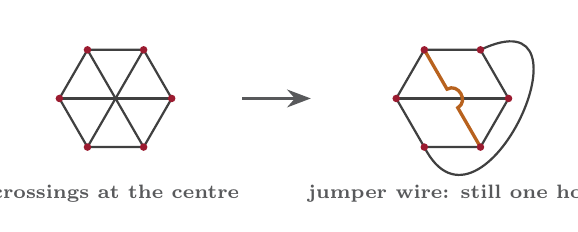
\begin{tikzpicture}[scale=0.62]
    \useasboundingbox (-1.8,-2.15) rectangle (8.9,1.45);
  \begin{scope}
    \foreach \a in {0,60,...,300} \coordinate (h\a) at (\a:1.15);
    \draw[black!75, thick] (h0) -- (h60) -- (h120) -- (h180) -- (h240) -- (h300) -- cycle;
    \draw[black!75, thick] (h0) -- (h180); \draw[black!75, thick] (h60) -- (h240);
    \draw[black!75, thick] (h120) -- (h300);
    \foreach \a in {0,60,...,300} \fill[metured] (h\a) circle (2.2pt);
    \node[ttl] at (0,-1.95) {crossings at the centre};
  \end{scope}
  \draw[bigarr] (2.6,0) -- (4.0,0);
  \begin{scope}[xshift=6.9cm]
    \hexhop
    \node[ttl] at (0,-1.95) {jumper wire: still one hop};
  \end{scope}
\end{tikzpicture}
\end{center}

%==============================================================
\section{Trees}

\begin{definitionbox}{Tree}
Let $G$ be a connected graph. A subgraph $T$ of $G$ is a \textbf{tree} if
\begin{enumerate}
  \item $T$ contains all the nodes of $G$,
  \item $T$ is connected, and
  \item $T$ contains no loops.
\end{enumerate}
\end{definitionbox}

\begin{examplebox}[Example 9.1 --- trees of the bridge graph]
Which of the green subgraphs are trees?
\begin{center}
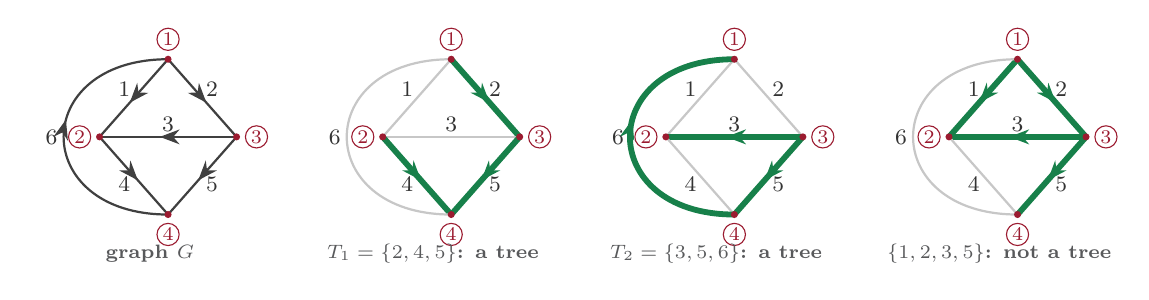
\begin{tikzpicture}[scale=0.58]
  \begin{scope}
    \bridgecoords \bridgegraph
    \node[ttl] at (-0.4,-2.55) {graph $G$};
  \end{scope}
  \begin{scope}[xshift=6.2cm]
    \bridgecoords \bridgesub{faintbr}{treebr}{faintbr}{treebr}{treebr}{faintbr}
    \node[ttl] at (-0.4,-2.55) {$T_1 = \{2, 4, 5\}$: a tree};
  \end{scope}
  \begin{scope}[xshift=12.4cm]
    \bridgecoords \bridgesub{faintbr}{faintbr}{treebr}{faintbr}{treebr}{treebr}
    \node[ttl] at (-0.4,-2.55) {$T_2 = \{3, 5, 6\}$: a tree};
  \end{scope}
  \begin{scope}[xshift=18.6cm]
    \bridgecoords \bridgesub{treebr}{treebr}{treebr}{faintbr}{treebr}{faintbr}
    \node[ttl] at (-0.4,-2.55) {$\{1, 2, 3, 5\}$: not a tree};
  \end{scope}
\end{tikzpicture}
\end{center}
$T_1$ and $T_2$ reach all four nodes, are connected and have no loop. The set
$\{1, 2, 3, 5\}$ contains the loop of branches 1, 2, 3, so it is not a tree. A graph has many
trees.
\end{examplebox}

\begin{ideabox}[A tree has $n-1$ branches]
Build the tree one branch at a time, starting from a single node. Each new branch must reach
a new node: a branch between two nodes already reached would close a loop. All $n$ nodes
must be reached, so the tree has exactly $n-1$ branches. The other $b - n + 1$ branches are
left out.
\end{ideabox}

%==============================================================
\section{Cutsets}

\begin{definitionbox}{Cutset}
Let $G$ be a connected graph. A set $C$ of branches is a \textbf{cutset} if
\begin{enumerate}
  \item removing all the branches of $C$ leaves the graph unconnected, and
  \item removing all the branches of $C$ except any one of them leaves it connected.
\end{enumerate}
\end{definitionbox}

The second condition makes the cutset minimal: every branch in it is needed. Minimal does not
mean fewest branches; cutsets of the same graph can have different sizes.

\begin{examplebox}[Example 9.2 --- cutsets of a figure-eight graph]
In each panel the removed branches are deleted; look at what is left.
\begin{center}
\tikzset{backbr/.style={ctree, line width=2.2pt}}
\begin{tabular}{@{}c@{\hspace{6mm}}c@{}}
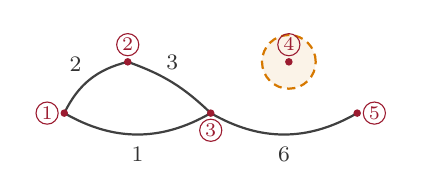
\begin{tikzpicture}[scale=0.62]
  \useasboundingbox (-3.75,-1.0) rectangle (3.75,1.75);
  \eightcoords \pieceP \eightsub{plainbr}{plainbr}{plainbr}{cutaway}{cutaway}{plainbr}{cutaway}
\end{tikzpicture}
&
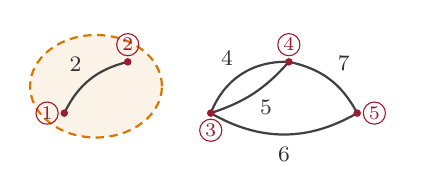
\begin{tikzpicture}[scale=0.62]
  \useasboundingbox (-3.75,-1.0) rectangle (3.75,1.75);
  \eightcoords \pieceLT \eightsub{cutaway}{plainbr}{cutaway}{plainbr}{plainbr}{plainbr}{plainbr}
\end{tikzpicture}\\[-1pt]
{\small $C_1 = \{4, 5, 7\}$: node \nd4 cut off} & {\small $C_2 = \{1, 3\}$: nodes \nd1, \nd2 cut off}\\[8pt]
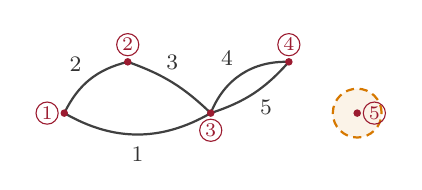
\begin{tikzpicture}[scale=0.62]
  \useasboundingbox (-3.75,-1.0) rectangle (3.75,1.75);
  \eightcoords \pieceR \eightsub{plainbr}{plainbr}{plainbr}{plainbr}{plainbr}{cutaway}{cutaway}
\end{tikzpicture}
&
\begin{tikzpicture}[scale=0.62]
  \useasboundingbox (-3.75,-1.0) rectangle (3.75,1.75);
  \eightcoords \pieceLTM \piecePR \eightsub{backbr}{plainbr}{cutaway}{cutaway}{cutaway}{cutaway}{plainbr}
\end{tikzpicture}\\[-1pt]
{\small $C_3 = \{6, 7\}$: node \nd5 cut off} & {\small $\{1, 3, 4, 5, 6\}$ with \textcolor{ctree}{1} put back: still two pieces}
\end{tabular}
\end{center}
For $C_1$: removing branches 4, 5, 7 cuts off node~\nd4, so condition~1 holds. Putting back
any one of them reaches node~\nd4 again, so condition~2 holds. $C_2$ and $C_3$ are checked
the same way. With all branches back, the dashed closed surface around the cut-off
piece crosses exactly the branches of the cutset.

The set $\{1, 3, 4, 5, 6\}$ is \emph{not} a cutset. Removing it leaves three pieces. With
branch~1 put back, the graph is still unconnected, so condition~2 fails. Branches 1 and 3 are
not needed: $\{4, 5, 6\}$ alone is a cutset.

The set $\{4, 6\}$ is not a cutset either, but for the opposite reason. Removing it leaves
the graph connected, since branch~5 still joins nodes \nd3 and \nd4, so condition~1 fails.
Branches 4 and 5 are parallel: both join \nd3 and \nd4. A closed surface that crosses one of
them crosses the other too. So parallel branches are in a cutset together or not at all.
\end{examplebox}

\textbf{KCL on a cutset.} A cutset splits the graph into two parts. A closed surface around
one part crosses exactly the branches of the cutset. So by KCL on that closed surface, the
currents of the cutset branches add up to zero (each with $+$ if it leaves the surface, $-$
if it enters).

Take the branch currents below, in the arrow directions. They satisfy KCL at every node.
Consider the cutset $\{4, 5, 6\}$, with the surface around nodes \nd4 and \nd5.
\begin{center}
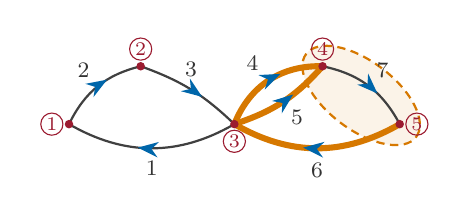
\begin{tikzpicture}[scale=0.7, baseline=(eM)]
  \useasboundingbox (-3.75,-1.0) rectangle (3.75,1.75);
  \eightcoords \piecePR
  \eightI{plainbr}{plainbr}{plainbr}{cutbr}{cutbr}{cutbr}{plainbr}
\end{tikzpicture}
\qquad
\eightItable
\end{center}
Current $\Icol{i_6}$ leaves the surface; $\Icol{i_4}$ and $\Icol{i_5}$ enter it:
\[
  \Icol{i_6} - \Icol{i_4} - \Icol{i_5} = 3 - 1 - 2 = 0.
\]
This is the sum of KCL at nodes \nd4 and \nd5:
$(\Icol{i_7} - \Icol{i_4} - \Icol{i_5}) + (\Icol{i_6} - \Icol{i_7}) = 0$. The current
$\Icol{i_7}$ is inside the surface and cancels.

%==============================================================
\section{Fundamental cutsets}

Fix a tree $T$ of a connected graph $G$. The branches of $G$ that are not in $T$ form the
\textbf{co-tree}. Now pick one tree branch $\beta$ and remove it. The tree falls into two
parts. The branches of $G$ that join these two parts form a cutset.

\begin{definitionbox}{Fundamental cutset}
The \textbf{fundamental cutset} of a tree branch $\beta$ is
\begin{itemize}
  \item $\beta$ plus the co-tree branches that join the two parts of the tree;
  \item it contains only one tree branch, $\beta$;
  \item its direction is that of $\beta$.
\end{itemize}
\end{definitionbox}

It has only one tree branch: every other tree branch lies inside one of the two parts, so it
does not join them. For the direction, draw the closed surface around one part. If $\beta$
leaves the surface, the cutset points out of the surface; if $\beta$ enters, it points in. In
KCL a branch counts $+$ if it crosses the surface the same way as $\beta$, and $-$ otherwise.

\begin{examplebox}[Example 9.3 --- fundamental cutsets and KCL]
The graph $G$ has $n = 4$ nodes and $b = 6$ branches. Take the tree $\{1, 3, 6\}$
(green, $n - 1 = 3$ branches). The co-tree is $\{2, 4, 5\}$ ($b - n + 1 = 3$ branches).
\begin{center}
\begin{minipage}[c]{0.42\linewidth}
\centering
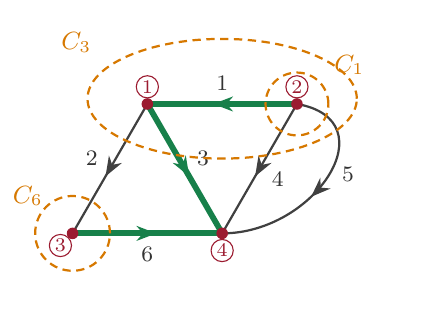
\begin{tikzpicture}[scale=0.95]
  \useasboundingbox (-2.6,-0.75) rectangle (2.5,2.75);
  \tgcoords \tgtree
  \draw[surf] (g2) circle (0.42);                \node[font=\small, text=cvolt] at (1.7,2.25) {$C_1$};
  \draw[surf] (0,1.8) ellipse (1.8 and 0.8);  \node[font=\small, text=cvolt] at (-1.95,2.55) {$C_3$};
  \draw[surf] (g3) circle (0.5);                 \node[font=\small, text=cvolt] at (-2.6,0.5) {$C_6$};
\end{tikzpicture}
\end{minipage}%
\begin{minipage}[c]{0.56\linewidth}
\centering\small
\renewcommand{\arraystretch}{1.3}
\setlength{\tabcolsep}{4pt}
\begin{tabular}{@{}c l l@{}}
\toprule
tree br. & cutset & KCL\\
\midrule
1 & $\{1, 4, 5\}$    & $\Icol{i_1} + \Icol{i_4} + \Icol{i_5} = 0$\\
3 & $\{3, 2, 4, 5\}$ & $\Icol{i_3} + \Icol{i_2} + \Icol{i_4} + \Icol{i_5} = 0$\\
6 & $\{6, 2\}$       & $\Icol{i_6} - \Icol{i_2} = 0$\\
\bottomrule
\end{tabular}
\end{minipage}
\end{center}
Each surface encloses one of the two parts left after removing a tree branch. For $C_3$:
removing branch~3 leaves the parts $\{\nd1, \nd2\}$ and $\{\nd3, \nd4\}$. Branches
3, 2, 4, 5 join them, and all four go from the upper part to the lower part, the same way
as branch~3: every term has $+$.
\end{examplebox}

\begin{ideabox}[KCL on the fundamental cutsets]
A tree gives $n-1$ fundamental cutsets, so $n-1$ KCL equations. They are independent: each
equation contains its own tree branch current, which appears in no other equation.
\end{ideabox}

\textbf{Branch currents from co-tree currents.} We can relate every branch current to the
co-tree currents. A co-tree current is itself. Each fundamental cutset has one tree branch,
so its KCL gives that tree branch current in terms of co-tree currents. For $G$:
\[
  \Icol{i_1} = -\Icol{i_4} - \Icol{i_5}, \quad
  \Icol{i_3} = -\Icol{i_2} - \Icol{i_4} - \Icol{i_5}, \quad
  \Icol{i_6} = \Icol{i_2} .
\]
So the $b - n + 1$ co-tree currents fix every branch
current, like mesh currents.

\textbf{Matrix form.} The fundamental cutset equations can be collected in the
\textbf{fundamental cutset matrix} $Q$: one row per tree branch, one column per branch. An
entry is $+1$ or $-1$ if the branch is in the cutset, in the same or the opposite direction,
and $0$ otherwise. For $G$:
\[
  Q = \brmat{Qn}{1, 3, 6}{\Qrows}{\foreach \j in {1,3,6} {\colbox{Qn}{\j}{ctree}}},
  \qquad Q\Icol{\mathbf{i}} = \mathbf{0} \quad (\text{like } A\Icol{\mathbf{i}} = \mathbf{0}).
\]
The tree columns (boxed) form an identity, so the rows are independent. The relation above, in
matrix form, is $\Icol{\mathbf{i}} = B^T\Icol{\mathbf{i}_C}$ with
$\Icol{\mathbf{i}_C} = [\Icol{i_2}\ \Icol{i_4}\ \Icol{i_5}]^T$, like
$\Icol{\mathbf{i}} = M^T\Icol{\mathbf{i}_M}$. Its transpose $B$ comes back with the
fundamental loops.

%==============================================================
\section{Fundamental loops}

Fix a tree $T$ of a connected graph $G$ and pick one co-tree branch. Adding it to the tree
closes exactly one loop: the co-tree branch plus the tree path between its two ends.

\begin{definitionbox}{Fundamental loop}
The \textbf{fundamental loop} of a co-tree branch is
\begin{itemize}
  \item that co-tree branch plus the tree path between its ends;
  \item it contains only one co-tree branch;
  \item its direction is that of the co-tree branch.
\end{itemize}
\end{definitionbox}

\begin{examplebox}[Example 9.4 --- fundamental loops and KVL]
Same graph and tree as in Example~9.3. Each co-tree branch closes one loop. Walk it in the
direction of its co-tree branch: a branch voltage counts $+$ if its arrow points along the
walk, $-$ if against.
\begin{center}
\begin{tabular}{@{}c@{\hspace{0.5cm}}c@{\hspace{0.5cm}}c@{}}
\begin{tabular}[t]{@{}c@{}}
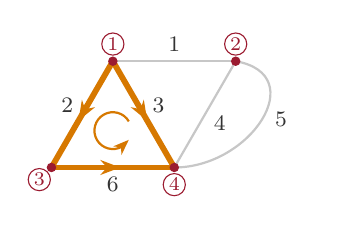
\begin{tikzpicture}[scale=0.78]
  \tgcoords \tgraph{faintbr}{hlbr}{hlbr}{faintbr}{faintbr}{hlbr}
  \loopccw{-1}{0.6}
\end{tikzpicture}\\[-2pt]
{\scriptsize\bfseries\color{metugray} loop of 2: $\{2, 6, 3\}$}\\[1pt]
{\small $\Vcol{v_2} + \Vcol{v_6} - \Vcol{v_3} = 0$}
\end{tabular}
&
\begin{tabular}[t]{@{}c@{}}
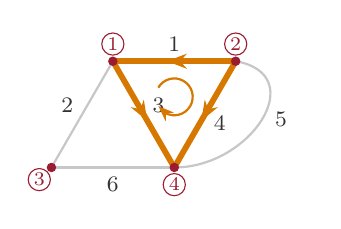
\begin{tikzpicture}[scale=0.78]
  \tgcoords \tgraph{hlbr}{faintbr}{hlbr}{hlbr}{faintbr}{faintbr}
  \loopcw{0}{1.15}
\end{tikzpicture}\\[-2pt]
{\scriptsize\bfseries\color{metugray} loop of 4: $\{4, 3, 1\}$}\\[1pt]
{\small $\Vcol{v_4} - \Vcol{v_3} - \Vcol{v_1} = 0$}
\end{tabular}
&
\begin{tabular}[t]{@{}c@{}}
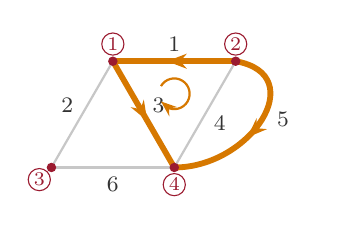
\begin{tikzpicture}[scale=0.78]
  \tgcoords \tgraph{hlbr}{faintbr}{hlbr}{faintbr}{hlbr}{faintbr}
  \loopcw[0.25]{0}{1.2}
\end{tikzpicture}\\[-2pt]
{\scriptsize\bfseries\color{metugray} loop of 5: $\{5, 3, 1\}$}\\[1pt]
{\small $\Vcol{v_5} - \Vcol{v_3} - \Vcol{v_1} = 0$}
\end{tabular}
\end{tabular}
\end{center}
\end{examplebox}

\begin{ideabox}[KVL on the fundamental loops]
A tree gives $b - n + 1$ fundamental loops, so $b - n + 1$ KVL equations. They are
independent: each equation contains its own co-tree branch voltage, which appears in no
other equation.
\end{ideabox}

\textbf{Branch voltages from tree voltages.} We can relate every branch voltage to the tree
voltages. A tree voltage is itself. Each fundamental loop has one co-tree branch, so its KVL
gives that co-tree branch voltage in terms of tree voltages. For $G$:
\[
  \Vcol{v_2} = \Vcol{v_3} - \Vcol{v_6}, \quad
  \Vcol{v_4} = \Vcol{v_1} + \Vcol{v_3}, \quad
  \Vcol{v_5} = \Vcol{v_1} + \Vcol{v_3} .
\]
So the $n - 1$ tree voltages fix every branch voltage, like
node voltages.

\textbf{Matrix form.} The fundamental loop equations are collected in the \textbf{fundamental
loop matrix} $B$: one row per co-tree branch; an entry is $+1$ or $-1$ if the branch is in the
loop, along or against its direction. It is the same $B$ as in
$\Icol{\mathbf{i}} = B^T\Icol{\mathbf{i}_C}$:
\[
  B = \brmat{Bn}{2, 4, 5}{\Brows}{\foreach \j in {2,4,5} {\colbox{Bn}{\j}{cvolt}}},
  \qquad B\Vcol{\mathbf{v}} = \mathbf{0} \quad (\text{like } M\Vcol{\mathbf{v}} = \mathbf{0}).
\]
The relation above, in matrix form, is $\Vcol{\mathbf{v}} = Q^T\Vcol{\mathbf{v}_T}$ with
$\Vcol{\mathbf{v}_T} = [\Vcol{v_1}\ \Vcol{v_3}\ \Vcol{v_6}]^T$, like
$\Vcol{\mathbf{v}} = A^T\Vcol{\mathbf{e}}$. Finally $QB^T = \mathbf{0}$, like
$AM^T = \mathbf{0}$.

%==============================================================
\section{Matrix form side by side}

\begin{center}
\renewcommand{\arraystretch}{1.25}
\begin{tabular}{@{}l l l@{}}
\toprule
 & incidence / mesh & fundamental cutset / loop\\
\midrule
KCL & $A\Icol{\mathbf{i}} = \mathbf{0}$ & $Q\Icol{\mathbf{i}} = \mathbf{0}$\\
KVL & $M\Vcol{\mathbf{v}} = \mathbf{0}$ & $B\Vcol{\mathbf{v}} = \mathbf{0}$\\
$n-1$ voltages & $\Vcol{\mathbf{v}} = A^T\Vcol{\mathbf{e}}$ (node voltages)
  & $\Vcol{\mathbf{v}} = Q^T\Vcol{\mathbf{v}_T}$ (tree voltages)\\
$b-n+1$ currents & $\Icol{\mathbf{i}} = M^T\Icol{\mathbf{i}_M}$ (mesh currents)
  & $\Icol{\mathbf{i}} = B^T\Icol{\mathbf{i}_C}$ (co-tree currents)\\
orthogonality & $AM^T = \mathbf{0}$ & $QB^T = \mathbf{0}$\\
works for & $A$: any; $M$: planar, nonseparable & any connected graph\\
\bottomrule
\end{tabular}
\end{center}
A circuit has $2b$ branch unknowns. A tree reduces them: the $n-1$ \textbf{tree branch
voltages} fix every branch voltage (like node voltages), and the $b-n+1$ \textbf{co-tree branch
currents} fix every branch current (like mesh currents), for any connected graph.


%==============================================================
\section{Any connected graph}

The tree is the key, and every connected graph has one. Its $n-1$ tree branches give the
KCL equations, and its $b-n+1$ co-tree branches give the KVL equations. No drawing is needed. This works for nonplanar graphs, and it is also the fix for separable
graphs met earlier.

\begin{examplebox}[Example 9.5 --- the separable graph]
Two loops joined only at node \nd1: $n = 5$, $b = 6$. Take the tree $\{1, 2, 4, 5\}$
(green, $n - 1 = 4$). The co-tree is $\{3, 6\}$ ($b - n + 1 = 2$).
\begin{center}\small
\renewcommand{\arraystretch}{1.15}\setlength{\tabcolsep}{3pt}
\begin{minipage}[c]{0.24\linewidth}
\centering
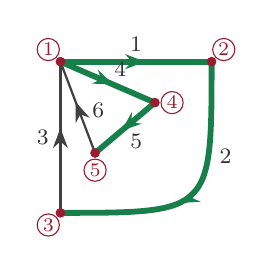
\begin{tikzpicture}[scale=0.8]
  \sepcoords \septree
\end{tikzpicture}
\end{minipage}%
\begin{minipage}[c]{0.34\linewidth}
\centering
\begin{tabular}{@{}c l l@{}}
\toprule
tree br. & cutset & KCL\\
\midrule
1 & $\{1, 3\}$ & $\Icol{i_1} - \Icol{i_3} = 0$\\
2 & $\{2, 3\}$ & $\Icol{i_2} - \Icol{i_3} = 0$\\
4 & $\{4, 6\}$ & $\Icol{i_4} - \Icol{i_6} = 0$\\
5 & $\{5, 6\}$ & $\Icol{i_5} - \Icol{i_6} = 0$\\
\bottomrule
\end{tabular}
\end{minipage}%
\begin{minipage}[c]{0.42\linewidth}
\centering
\begin{tabular}{@{}c l@{}}
\toprule
co-tree br. & KVL on its loop\\
\midrule
3 & $\Vcol{v_3} + \Vcol{v_1} + \Vcol{v_2} = 0$\\
6 & $\Vcol{v_6} + \Vcol{v_4} + \Vcol{v_5} = 0$\\
\bottomrule
\end{tabular}
\end{minipage}
\end{center}
The two fundamental loops are the outer loop and the inner triangle. The KCL equations give
$\Icol{i_1} = \Icol{i_2} = \Icol{i_3}$ and $\Icol{i_4} = \Icol{i_5} = \Icol{i_6}$: one current
for each loop. In total $4 + 2 = 6 = b$ independent equations. Node~\nd1 causes no trouble.
\end{examplebox}

%==============================================================
\section*{Summary}
\addcontentsline{toc}{section}{Summary}

\begin{itemize}
  \item A \textbf{tree} of a connected graph contains all nodes, is connected and has no
        loop. It has $n-1$ branches; the other $b-n+1$ form the \textbf{co-tree}.
  \item A \textbf{cutset} is a minimal set of branches whose removal cuts the graph in two.
        KCL holds on every cutset: it is KCL on a closed surface.
  \item Each tree branch has a \textbf{fundamental cutset}: it and some co-tree branches.
        These give $n-1$ independent KCL equations. Every branch current follows from the co-tree currents.
  \item Each co-tree branch has a \textbf{fundamental loop}: it and a tree path. These give
        $b-n+1$ independent KVL equations. Every branch voltage follows from the tree voltages.
\end{itemize}

\end{document}
